\subsection{Short introduction to nuclear and particle physics}
In order to understand the notions of half life period and nuclear fission we need to
give a short introduction into nuclear and particle physics, herefore we follow \cite{Hooshyar}.
Let now in the following be $Z$ - atomic number,  $N$ - number of neutrons and  $A$ - the number of nucleons, also
called nucleon number, such that $A = Z + N$. The electric charge of the nucleus in ground state is $+Z e$.
It is common now to describe the so called nuclides with $_{Z}^{A}\textrm{Y}$.\\
The Forces that bind the nucleons in the nuclei contribute to the total mass of an atom in terms of the 
binding energy $\Delta E = \Delta M c^2$:
\begin{equation}
\Delta M = M_{tot.} - Z(M_p + M_e) - N M_n
\end{equation}
Where we used the proton, electron and neutron masses $M_p$, $M_e$ and $M_n$ 
(see figure~/ref{fig:bindingenergy}).
\begin{figure}[htpb]
    \centering
    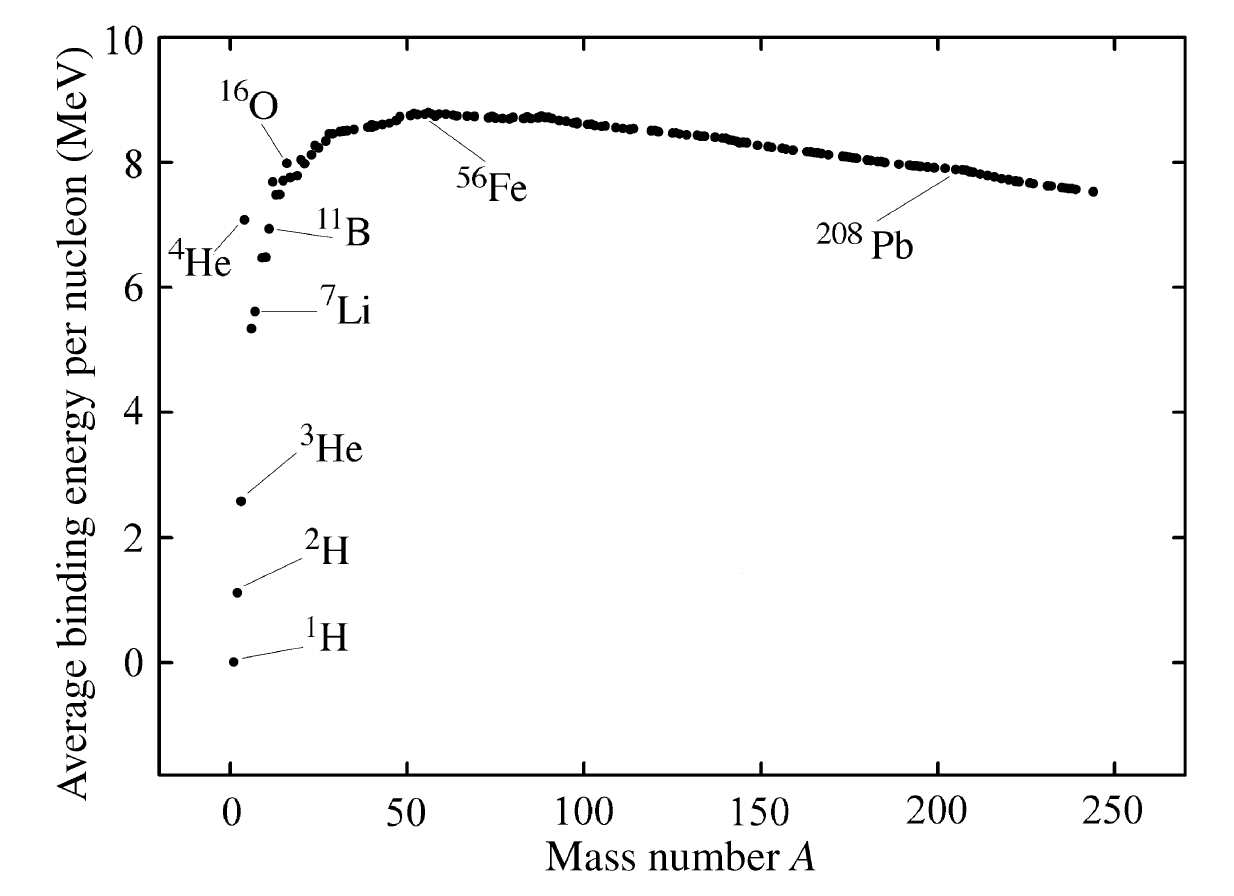
\includegraphics[width=0.8\linewidth]{figures/bindingenergy}
    \caption{Binding energies for nuclei that are stable or long-lived \cite{Hooshyar}.}
    \label{fig:bindingenergy}
\end{figure}
If we look at the distribution of stable nuclei (see figure~\ref{fig:nuclidmap}) we notice
that stable nuclei only occur in a very narrow band, other nuclei are unstable and decay sponatneously.
The decay is characerized by a \textit{decay constant} $\lambda$, which is related to the activity $\mathcal{A}$
by 
\begin{equation}\label{eq:decay}
    \mathcal{A} = -\frac{\partial N}{\partial t} = \lambda N 
\end{equation}
Where the activity $\mathcal{A}$ is typically given in Bequerel: $1 \textrm{Bq}= \textrm{decay}\cdot s^{-1}$ 
The solution to the differential equation in \eqref{eq:decay} yields:
\begin{equation}
    \mathcal{A}(t) = \lambda N_0 \exp(-\lambda t)
\end{equation}
with the initial condition $N_0 := N(t=t_0)$. 
The probability of an Atom to decay after time $t$ is thus:
\begin{equation}
    \mathcal{P}(t) = \int_{0}^{t}\lambda \exp(-\lambda t')\mathrm{d}t' = 1 -  \exp(-\lambda t)  \quad
    \textrm{with} \quad \int_{0}^{\infty}\lambda \exp(-\lambda t')\mathrm{d}t' = 1
\end{equation}
such that the probability density is $f(t) = \lambda \exp(-\lambda t)$.
Hence we can calculate the expectation value of a random variable $t$ within the probability space
$\Omega$ with the measure  $\mathcal{P}$:
\begin{equation}
    \tau := E[t] = \int_{0}^{\infty} t \lambda \exp(-\lambda t) \mathrm{d}t 
    =\lim_{t \rightarrow \infty}\left[ \frac{exp(-\lambda t) (1-\lambda t) - 1 }{\lambda} \right] 
= \frac{1}{\lambda}
\end{equation}
The half-life $t_{1/2}$ is obviously connected by $t_{1/2}= -\mathrm{log}(2)/ \lambda = - \tau \mathrm{log}(2)$.
\begin{figure}[htpb]
    \centering
    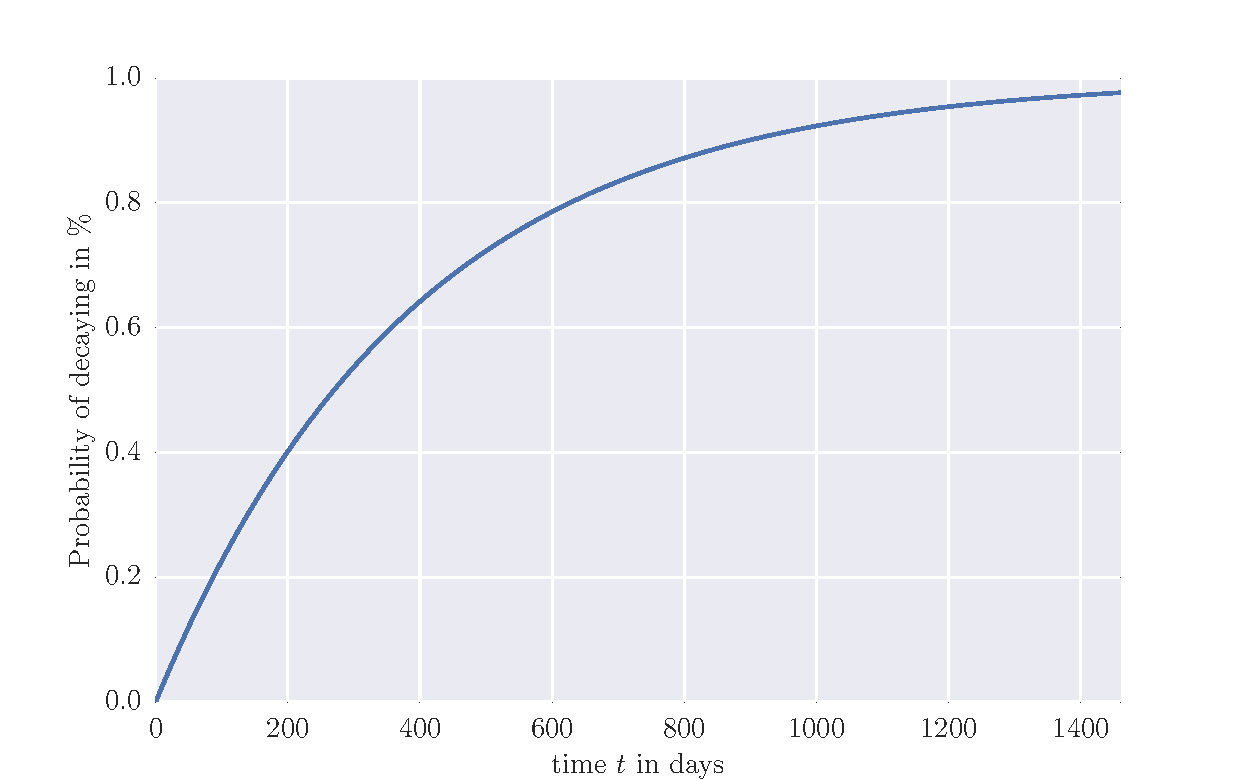
\includegraphics[width=0.9\linewidth]{analysis/figures/halflife}
    \caption{Probability $\mathcal{P}(t) = 1 -  \exp(-\lambda t)$ of an atom to decay after time $t$.
        Here we chose as an example the decay of Cs $\rightarrow$ Fe with $t_{1/2}=270$ over a timerange
    of 4 years.}
    \label{fig:decay}
\end{figure}
\clearpage
\subsubsection{Semi-Empirical Mass Formula: The Liquid Drop Model}
\begin{figure}[htpb]
    \centering
    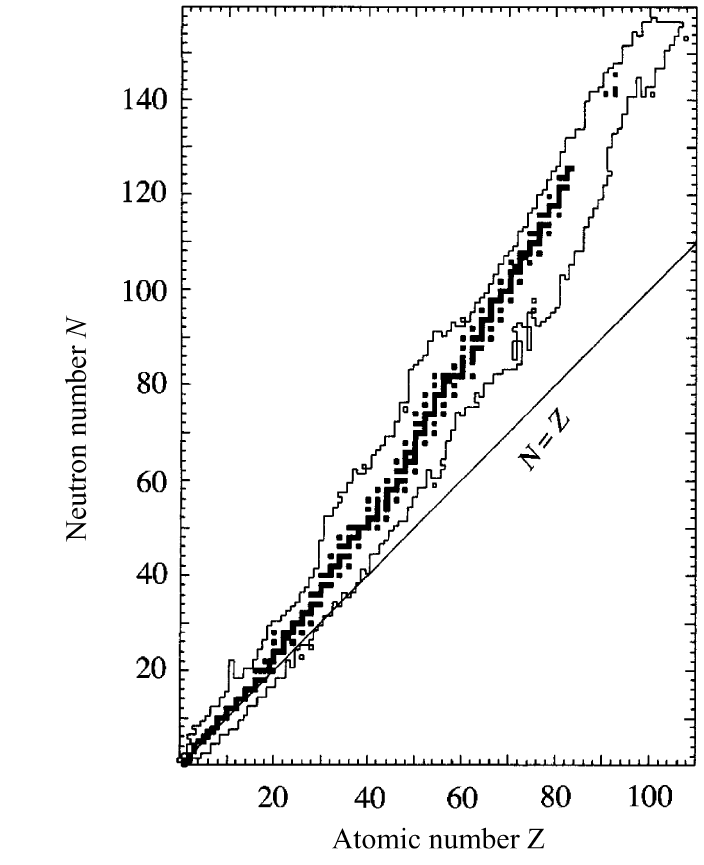
\includegraphics[width=0.6\linewidth]{figures/nuclidmap}
    \caption{Nuclid map of stable nuclei \cite{Hooshyar}: The squares are the long-lived nuclei
    occuing in nature; otherknown nuclei lie within the jagged lines and are unstable.}
    \label{fig:nuclidmap}
\end{figure}
\label{ssub:Semi-Empirical Mass Formula: The Liquid Drop Model}
We continue following \cite{Hooshyar}. We now approach an theoretic model which contains constants which
have to be fitted with experiments, thats why its called semi-empirical. 
The model was first established by Weizsäcker and will yield a 
good approximation for the atomic masses. The model is built upon the following assumptions, which turn
out to be valid in the regime we are looking at:
\begin{enumerate}
    \item The interior mass densities are approximately equal,
    \item their total binding energies are approximately proportional to their masses.
\end{enumerate}
This shows why the model is called ``Liquid Drop Model'', since (1.) relates to the equality of densities
of drops and (2) to the proportionality of latent heats of vaporization to the masses of a drops. 
\clearpage


